%!TeX root=../../tcc.tex

%% ------------------------------------------------------------------------- %%
\chapter{Ordenação cinética}
Considere o seguinte problema cinético. São dados $n$ pares de
valores. Cada par $(x_0, v)$ representa um valor que está mudando
linearmente com o tempo. Num instante arbitrário $t \geq 0$, o valor
correspondente ao par $(x_0, v)$ é $x_0 + tv$. O objetivo é
responder consultas do tipo: para um certo $i$, com $1 \leq i \leq
n$, quem é o $i$-ésimo maior valor da coleção no instante corrente.

Por exemplo, se tivermos quatro elementos na coleção, digamos
$\left(6, -\frac{1}{2}\right)$, $(5, 0)$, $\left(3,
\frac{1}{4}\right)$ e $\left(0, \frac{4}{3}\right)$, podemos
representar essa coleção como na figura \ref{fig:ordenacao:exemplo}.

\begin{figure}[H]
    \centering
    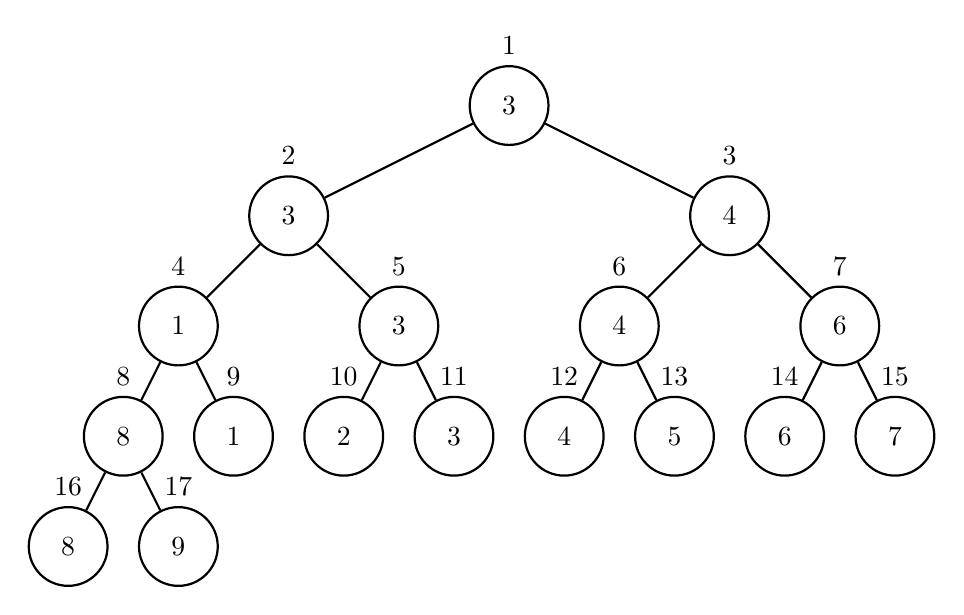
\begin{tikzpicture}[thick, scale=0.7]
        \node[label={1},circle,draw,minimum size=1cm]
        (1) at (0,0) {$3$};
        \node[label={2},circle,draw,minimum size=1cm]
        (2) at (-4,-2) {$3$};
        \node[label={3},circle,draw,minimum size=1cm]
        (3) at (4,-2) {$4$};
        \node[label={4},circle,draw,minimum size=1cm]
        (4) at (-6,-4) {$1$};
        \node[label={5},circle,draw,minimum size=1cm]
        (5) at (-2,-4) {$3$};
        \node[label={6},circle,draw,minimum size=1cm]
        (6) at (2,-4) {$4$};
        \node[label={7},circle,draw,minimum size=1cm]
        (7) at (6,-4) {$6$};
        \node[label={8},circle,draw,minimum size=1cm]
        (8) at (-7,-6) {$8$};
        \node[label={9},circle,draw,minimum size=1cm]
        (9) at (-5,-6) {$1$};
        \node[label={10},circle,draw,minimum size=1cm]
        (10) at (-3,-6) {$2$};
        \node[label={11},circle,draw,minimum size=1cm]
        (11) at (-1,-6) {$3$};
        \node[label={12},circle,draw,minimum size=1cm]
        (12) at (1,-6) {$4$};
        \node[label={13},circle,draw,minimum size=1cm]
        (13) at (3,-6) {$5$};
        \node[label={14},circle,draw,minimum size=1cm]
        (14) at (5,-6) {$6$};
        \node[label={15},circle,draw,minimum size=1cm]
        (15) at (7,-6) {$7$};
        \node[label={16},circle,draw,minimum size=1cm]
        (16) at (-8,-8) {$8$};
        \node[label={17},circle,draw,minimum size=1cm]
        (17) at (-6,-8) {$9$};

        \draw[thick] (1) -- (2);
        \draw[thick] (2) -- (4);
        \draw[thick] (4) -- (8);
        \draw[thick] (4) -- (9);
        \draw[thick] (8) -- (16);
        \draw[thick] (8) -- (17);
        \draw[thick] (2) -- (5);
        \draw[thick] (5) -- (10);
        \draw[thick] (5) -- (11);
        \draw[thick] (1) -- (3);
        \draw[thick] (3) -- (6);
        \draw[thick] (3) -- (7);
        \draw[thick] (6) -- (12);
        \draw[thick] (6) -- (13);
        \draw[thick] (7) -- (14);
        \draw[thick] (7) -- (15);
    \end{tikzpicture}
    \caption[Representação da estrutura torneio]{Torneio com $9$
        elementos em que $3$ é o elemento com valor máximo.}
    \label{fig:torneio:exemplo}
\end{figure}

\newpage

Queremos dar suporte às seguintes operações:
\begin{itemize}
    \item \textsc{advance}$(t)$ $\rightarrow$ avança o tempo
    corrente para $t$;
    \item \textsc{change}$(j, v)$ $\rightarrow$ altera a
    velocidade do elemento $j$ para $v$;
    \item \textsc{query\_kth}$(i)$ $\rightarrow$ devolve o
    elemento cujo valor é o $i$-ésimo maior no instante atual.
\end{itemize}

%!TeX root=./ordenacao.tex

%% ------------------------------------------------------------------------- %%


\section{Lista ordenada cinética}
\label{sec:lista}
Um jeito natural de resolver o problema da ordenação cinética é por
meio de uma lista ordenada cinética, que é manter um vetor com os
elementos dados em ordem decrescente do valor no instante atual.

Inicialmente o vetor começa com os valores dos elementos no instante
$t = 0$, ou seja, com o valor $x_0$ de cada elemento, e este vetor é
ordenado em ordem decrescente.
Na verdade, o vetor pode armazenar não os valores, mas os índices dos elementos, e fazemos
ordenação indireta.
No caso de empates nos valores dos elementos, o desempate
será feito pela velocidade: se dois elementos, digamos $i$
e $j$, possuem o mesmo valor $x_0$, mas a velocidade de $i$ é maior
que a de $j$, então $i$ será tratado como se possuísse maior valor
que $j$ no instante inicial.
Esse mesmo critério de desempate será aplicado em todos os instantes e também em todos os
problemas daqui em diante.

\begin{figure}[H]
    \centering
    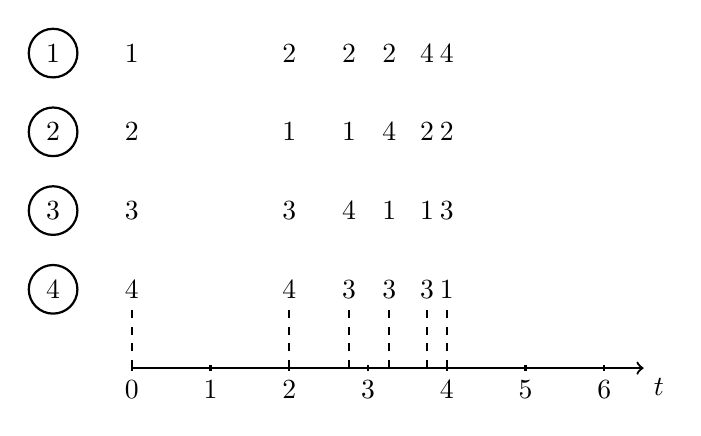
\begin{tikzpicture}[thick]
        \draw[thick,->] (0,0) -- (6.5,0) node[anchor=north west]
            {$t$};
%        \draw[thick,->] (0,0) -- (0,8) node[anchor=south east]
%            {valor$(t)$};
        \foreach \x in {0, 1,..., 6}
        \draw (\x cm,1pt) -- (\x cm,-1pt)
        node[anchor=north] {$\x$};
        \node[circle, draw] at (-1,1 cm) {$4$};
        \node[circle, draw] at (-1,2 cm) {$3$};
        \node[circle, draw] at (-1,3 cm) {$2$};
        \node[circle, draw] at (-1,4 cm) {$1$};

        \node at (0,1 cm) {$4$};
        \node at (0,2 cm) {$3$};
        \node at (0,3 cm) {$2$};
        \node at (0,4 cm) {$1$};

        \node at (2,1 cm) {$4$};
        \node at (2,2 cm) {$3$};
        \node at (2,3 cm) {$1$};
        \node at (2,4 cm) {$2$};

        \node at (2.76,1 cm) {$3$};
        \node at (2.76,2 cm) {$4$};
        \node at (2.76,3 cm) {$1$};
        \node at (2.76,4 cm) {$2$};

        \node at (3.27,1 cm) {$3$};
        \node at (3.27,2 cm) {$1$};
        \node at (3.27,3 cm) {$4$};
        \node at (3.27,4 cm) {$2$};

        \node at (3.75,1 cm) {$3$};
        \node at (3.75,2 cm) {$1$};
        \node at (3.75,3 cm) {$2$};
        \node at (3.75,4 cm) {$4$};

        \node at (4,1 cm) {$1$};
        \node at (4,2 cm) {$3$};
        \node at (4,3 cm) {$2$};
        \node at (4,4 cm) {$4$};


        \draw[dashed] (0, 0) -- (0, 0.8);
        \draw[dashed] (2, 0) -- (2, 0.8);
        \draw[dashed] (2.76, 0) -- (2.76, 0.8);
        \draw[dashed] (3.27, 0) -- (3.27, 0.8);
        \draw[dashed] (3.75, 0) -- (3.75, 0.8);
        \draw[dashed] (4, 0) -- (4, 0.8);


    \end{tikzpicture}
    \caption[Exemplo de trocas na lista ordenada]{Vetor com os índices dos elementos, ordenado
    pelos valores dos elementos no tempo $t = 0$ e suas
    alterações a medida que o tempo avança, para os quatro
    elementos da Figura~\ref{fig:ordenacao:exemplo}.}
    \label{fig:lista:vetores}
\end{figure}

Uma vez de posse do vetor ordenado com os valores iniciais
decrescentemente, construímos um certificado para cada par de
elementos consecutivos no vetor.
O $i$-ésimo certificado, denotado pelo par $(i, t)$, se refere ao par das posições $i$ e $i + 1$.
O valor $t$ consiste no instante de tempo em que o $i$-ésimo elemento
deixará de ter um valor maior que o valor do $(i + 1)$-ésimo
elemento do vetor, se esse instante for maior ou igual a 0, ou em
geral ao instante atual.
Do contrário, o valor $t$ consiste em $+\infty$.
O valor $t$ do certificado é o seu \textit{prazo de
validade}.

Esses prazos de validade determinam os \textit{eventos} que
potencialmente causarão modificações no vetor que mantém os
elementos ordenados pelo seu valor e, consequentemente, em alguns
certificados.

Esses $n - 1$ certificados são colocados em uma fila com
prioridades, com seu prazo de validade determinando a prioridade.
Estamos interessados nos certificados com menor prazo de validade.
Ou seja, a fila com prioridades pode ser implementada com um heap de
mínimo que usa os prazos de validade como chave.

Para descrever a implementação das três operações, precisamos
estabelecer o nome das variáveis usadas.
São elas:
\begin{enumerate}
    \item $n$: o número de elementos dados;
    \item $x_0$ e \textit{speed}: vetores com o valor e a velocidade
    inicial de cada um dos $n$ elementos;
    \item \now: instante atual.
    A variável \now\ será tratada como
    global, ou seja, será utilizada nas rotinas sem ser passada como
    argumento;
    \item \textit{sorted}: vetor com os índices dos $n$ elementos em
    ordem decrescente do seu valor no instante \textit{now};
%    \item \textit{indS}: vetor de $n$ posições; \textit{indS}[$j$]
%    guarda a posição em \textit{sorted} do elemento $j$;
    \item \textit{cert}: vetor com os $n-1$ certificados;
    \textit{cert}$[i]$ guarda o $i$-ésimo certificado, ou seja, o certificado
    entre $\sorted[i]$ e ${\sorted[i+1]}$, para~$1\leq i < n$;
    \item \textit{Q}: fila que guarda os inteiros $1, \ldots, n-1$,
    sendo \textit{cert}[$i$] a prioridade do inteiro $i$ na fila.
\end{enumerate}

\begin{figure}[H]
    \centering
    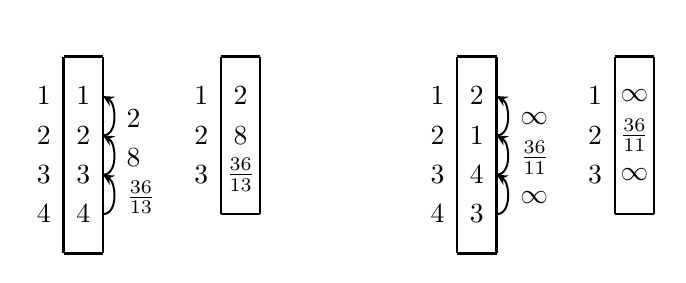
\begin{tikzpicture}[thick]
        \node at (0.5,0 cm) {$4$};
        \node at (0.5,0.5 cm) {$3$};
        \node at (0.5,1 cm) {$2$};
        \node at (0.5,1.5 cm) {$1$};

        \draw (0.75,-0.5) -- (0.75, 2);
        \draw (1.25,-0.5) -- (1.25, 2);
        \draw (0.75,-0.5) -- (1.25,-0.5);
        \draw (0.75, 2) -- (1.25, 2);
        \node at (1,0 cm) {$4$};
        \node at (1,0.5 cm) {$3$};
        \node at (1,1 cm) {$2$};
        \node at (1,1.5 cm) {$1$};

        \draw[->, shorten >= 0.1pt, shorten <= 0.1pt, >=stealth, line width=0.25mm]
        (1.25, 0) to[out=0,in=-30] node[right=1pt] {$\frac{36}{13}$} (1.25, 0.5);

        \draw[->, shorten >= 0.1pt, shorten <= 0.1pt, >=stealth, line width=0.25mm]
        (1.25, 0.5) to[out=0,in=-30] node[right=1pt] {$8$} (1.25, 1);

        \draw[->, shorten >= 0.1pt, shorten <= 0.1pt, >=stealth, line width=0.25mm]
        (1.25, 1) to[out=0,in=-30] node[right=1pt] {$2$} (1.25, 1.5);

        \node at (1,2.25 cm) {$\sorted$};

        \node at (2.5,0.5 cm) {$3$};
        \node at (2.5,1 cm) {$2$};
        \node at (2.5,1.5 cm) {$1$};

        \draw (2.75,0) -- (2.75, 2);
        \draw (3.25,0) -- (3.25, 2);
        \draw (2.75,0) -- (3.25,0);
        \draw (2.75, 2) -- (3.25, 2);
        \node at (3,0.5 cm) {$\frac{36}{13}$};
        \node at (3,1 cm) {$8$};
        \node at (3,1.5 cm) {$2$};

        \node at (3,2.25 cm) {$\cert$};

        \begin{scope}
            [shift={(5,0)}]
            \node at (0.5,0 cm) {$4$};
            \node at (0.5,0.5 cm) {$3$};
            \node at (0.5,1 cm) {$2$};
            \node at (0.5,1.5 cm) {$1$};

            \draw (0.75,-0.5) -- (0.75, 2);
            \draw (1.25,-0.5) -- (1.25, 2);
            \draw (0.75,-0.5) -- (1.25,-0.5);
            \draw (0.75, 2) -- (1.25, 2);
            \node at (1,0 cm) {$3$};
            \node at (1,0.5 cm) {$4$};
            \node at (1,1 cm) {$1$};
            \node at (1,1.5 cm) {$2$};

            \draw[->, shorten >= 0.1pt, shorten <= 0.1pt, >=stealth, line width=0.25mm]
            (1.25, 0) to[out=0,in=-30] node[right=1pt] {$\infty$} (1.25, 0.5);

            \draw[->, shorten >= 0.1pt, shorten <= 0.1pt, >=stealth, line width=0.25mm]
            (1.25, 0.5) to[out=0,in=-30] node[right=1pt] {$\frac{36}{11}$} (1.25, 1);

            \draw[->, shorten >= 0.1pt, shorten <= 0.1pt, >=stealth, line width=0.25mm]
            (1.25, 1) to[out=0,in=-30] node[right=1pt] {$\infty$} (1.25, 1.5);

            \node at (1,2.25 cm) {$\sorted$};

            \node at (2.5,0.5 cm) {$3$};
            \node at (2.5,1 cm) {$2$};
            \node at (2.5,1.5 cm) {$1$};

            \draw (2.75,0) -- (2.75, 2);
            \draw (3.25,0) -- (3.25, 2);
            \draw (2.75,0) -- (3.25,0);
            \draw (2.75, 2) -- (3.25, 2);
            \node at (3,0.5 cm) {$\infty$};
            \node at (3,1 cm) {$\frac{36}{11}$};
            \node at (3,1.5 cm) {$\infty$};

            \node at (3,2.25 cm) {$\cert$};

        \end{scope}
    \end{tikzpicture}
    \caption[Exemplo das estruturas utilizadas na lista ordenada]{Vetores $\sorted$ e $\cert$ para
        $\now = 0$ e $\now = 3$.
        O instante $t = \frac{36}{13}$ é quando as trajetórias dos elementos $3$ e $4$ se cruzam, e
        $t = \frac{36}{11}$ é quando as trajetórias dos elementos $1$ e $4$ se cruzam.}
    \label{fig:lista:variaveis}
\end{figure}



A interface da fila com prioridades que utilizaremos inclui as duas
seguintes operações:
\begin{enumerate}
    \item \textsc{minPQ}$(Q)$: devolve $i$ tal que
    \textit{cert}[$i$] é mínimo;
    \item \textsc{updatePQ}$(Q, i, t)$: altera a chave do
    $i$-ésimo certificado para $t$ e ajusta $Q$ de acordo.
\end{enumerate}

Note que não usaremos inserção ou remoção da fila com prioridades.

Para implementar a operação \textsc{change} de maneira eficiente, utilizaremos um vetor adicional
$\inds$ que guarda em $\inds[j]$ a posição em $\sorted$ do elemento $j$.
Utilizaremos $\textit{indS}$ pois, dado um elemento $j$, precisamos saber a posição $i$ do
elemento $j$ em $\sorted$ para recalcular os certificados relacionados com a posição $i$.
Para implementar a operação \textsc{updatePQ}$(Q, i, t)$ em tempo logarítmico no número de
elementos na fila $Q$, é necessário utilizar um vetor adicional \textit{indQ} que guarda em
\textit{indQ}$[i]$ a posição em $Q$ do $i$-ésimo certificado.

Com isso, a operação \textsc{advance}$(t)$, implementada no
Algoritmo~\ref{alg:lista-ordenada:advance}, segue uma ideia bem simples: enquanto
$t$ for maior que o prazo de validade do próximo evento, avançamos
\textit{now} para esse prazo de validade e tratamos esse evento.
Nos problemas seguintes, a operação \textsc{advance}$(t)$ será essencialmente a
mesma;
as únicas mudanças ocorrerão no tratamento de um evento.

\begin{algorithm}[H]
    \caption[Algoritmo \textsc{advance}]{Função \textsc{advance}.} \label{alg:lista-ordenada:advance}
\begin{algorithmic}[1]
    \Function{advance}{$t$}
        \If{$t < $ \now}
            \State \Return
        \EndIf
        \State $i \leftarrow \Call{minPQ}{$Q$}$
        \While{$t \geq$ \cert[$i$]}
            \State \now $~\leftarrow$ \cert[i]
            \State $\Call{event}$
            \State $i \leftarrow \Call{minPQ}{$Q$}$
        \EndWhile
        \State \now $~\leftarrow$ $t$
    \EndFunction
\end{algorithmic}
\end{algorithm}

Um evento está associado a um certificado $(i, t)$ que expira quando
$\now = t$.
O tratamento do evento correspondente ao certificado $(i, t)$ consiste em trocar de lugar os
índices das posições $i$ e $i + 1$ do vetor \textit{sorted}, recalcular o prazo de validade do
$(i-1)$-ésimo certificado se $i > 1$, e do $(i + 1)$-ésimo
certificado se $i < n - 1$.
O $i$-ésimo certificado também deve ser ajustado para $+\infty$.
Finalmente, é necessário fazer ajustes em $Q$, nas chaves dos certificados que sofreram
alteração.

Na implementação da operação \textsc{event}, utilizaremos a rotina
\textsc{update}$(i)$ para calcular o novo prazo de validade $t$ do
$i$-ésimo certificado, se $1 \leq i < n$, e fazer os devidos ajustes
em~$Q$.
Para calcular $t$, utilizaremos uma rotina chamada \textsc{expire}$(i,
j)$, que calcula o prazo de validade dos certificados entre os
elementos $i$ e $j$ no instante \now.
A rotina auxiliar \textsc{expire}$(i, j)$ não mudará para outros problemas, mantendo a
mesma definição.
As implementações estão nos Algoritmos~\ref{alg:lista-ordenada:update}
e~\ref{alg:lista-ordenada:evento} e a Figura~\ref{fig:lista:expire}
ilustra as atualizações feitas por essas rotinas.

\begin{algorithm}
    \caption{Função \textsc{update}.} \label{lista:update}
\begin{algorithmic}[1]
    \Function{update}{$i$}
        \If{$1 \leq i < n$}
            \State $t \leftarrow $ \Call{expire}{$i,i+1$}
            \State \Call{updatePQ}{$Q,i,t$}
        \EndIf
    \EndFunction
\end{algorithmic}
\end{algorithm}

\begin{algorithm}
    \caption{Função \textsc{event}.} \label{torneioi:evento}
    \begin{algorithmic}[1]
        \Function{event}{\nnull}
            \State $e \leftarrow  $ \Call{minPQ}{$Q$}
            \While{$e.\cert$ = \now}
                \State $j \leftarrow e.\lastmatch$
                \State $k \leftarrow 2\cdot \floor{\frac{j}{2}}
                + ((j + 1)\mod2)$ \Comment{adversário}
                \While{$j > 1$ \AND \Call{compare}{$j, k$}}
                    \State \torneio[$\floor{\frac{j}{2}}$]
                    $\leftarrow~$\torneio[$j$]
                    \State $\torneio[k].\lastmatch$ $\leftarrow k$
                    \State \Call{update}{$\torneio[k]$}
                    \State $j \leftarrow \floor{\frac{j}{2}}$
                    \State $k \leftarrow 2\cdot \floor{\frac{j}{2}}
                    + ((j + 1)\mod2)$ \Comment{adversário}
                \EndWhile
                \State $\torneio[j].\lastmatch \leftarrow j$
                \State \Call{update}{$\torneio[j]$}
                \State $e \leftarrow  $ \Call{minPQ}{$Q$}
            \EndWhile
        % \LineComment{swapHeap$(i, \floor{\frac{i}{2}})$ troca \heap[$i$] por \heap$\left[\floor{\frac{i}{2}}\right]$}
        \EndFunction
        \LineComment{\Call{compare}{$i, j$} retorna se o valor
        de $i$ é maior que o valor de $j$.}
    \end{algorithmic}
\end{algorithm}

\begin{figure}[H]
    \centering
    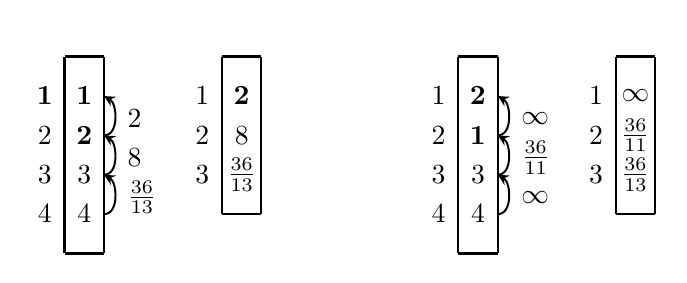
\begin{tikzpicture}[thick]
        \node at (0.5,0 cm) {$4$};
        \node at (0.5,0.5 cm) {$3$};
        \node at (0.5,1 cm) {$2$};
        \node at (0.5,1.5 cm) {\textbf{1}};

        \draw (0.75,-0.5) -- (0.75, 2);
        \draw (1.25,-0.5) -- (1.25, 2);
        \draw (0.75,-0.5) -- (1.25,-0.5);
        \draw (0.75, 2) -- (1.25, 2);
        \node at (1,0 cm) {$4$};
        \node at (1,0.5 cm) {$3$};
        \node at (1,1 cm) {$\textbf{2}$};
        \node at (1,1.5 cm) {$\textbf{1}$};

        \draw[->, shorten >= 0.1pt, shorten <= 0.1pt, >=stealth, line width=0.25mm]
        (1.25, 0) to[out=0,in=-30] node[right=1pt] {$\frac{36}{13}$} (1.25, 0.5);

        \draw[->, shorten >= 0.1pt, shorten <= 0.1pt, >=stealth, line width=0.25mm]
        (1.25, 0.5) to[out=0,in=-30] node[right=1pt] {$8$} (1.25, 1);

        \draw[->, shorten >= 0.1pt, shorten <= 0.1pt, >=stealth, line width=0.25mm]
        (1.25, 1) to[out=0,in=-30] node[right=1pt] {$2$} (1.25, 1.5);

        \node at (1,2.25 cm) {$\sorted$};

        \node at (2.5,0.5 cm) {$3$};
        \node at (2.5,1 cm) {$2$};
        \node at (2.5,1.5 cm) {$1$};

        \draw (2.75,0) -- (2.75, 2);
        \draw (3.25,0) -- (3.25, 2);
        \draw (2.75,0) -- (3.25,0);
        \draw (2.75, 2) -- (3.25, 2);
        \node at (3,0.5 cm) {$\frac{36}{13}$};
        \node at (3,1 cm) {$8$};
        \node at (3,1.5 cm) {$\textbf{2}$};

        \node at (3,2.25 cm) {$\cert$};

        \begin{scope}
            [shift={(5,0)}]
            \node at (0.5,0 cm) {$4$};
            \node at (0.5,0.5 cm) {$3$};
            \node at (0.5,1 cm) {$2$};
            \node at (0.5,1.5 cm) {$1$};

            \draw (0.75,-0.5) -- (0.75, 2);
            \draw (1.25,-0.5) -- (1.25, 2);
            \draw (0.75,-0.5) -- (1.25,-0.5);
            \draw (0.75, 2) -- (1.25, 2);
            \node at (1,0 cm) {$4$};
            \node at (1,0.5 cm) {$3$};
            \node at (1,1 cm) {$\textbf{1}$};
            \node at (1,1.5 cm) {$\textbf{2}$};

            \draw[->, shorten >= 0.1pt, shorten <= 0.1pt, >=stealth, line width=0.25mm]
            (1.25, 0) to[out=0,in=-30] node[right=1pt] {$\infty$} (1.25, 0.5);

            \draw[->, shorten >= 0.1pt, shorten <= 0.1pt, >=stealth, line width=0.25mm]
            (1.25, 0.5) to[out=0,in=-30] node[right=1pt] {$\frac{36}{11}$} (1.25, 1);

            \draw[->, shorten >= 0.1pt, shorten <= 0.1pt, >=stealth, line width=0.25mm]
            (1.25, 1) to[out=0,in=-30] node[right=1pt] {$\infty$} (1.25, 1.5);

            \node at (1,2.25 cm) {$\sorted$};

            \node at (2.5,0.5 cm) {$3$};
            \node at (2.5,1 cm) {$2$};
            \node at (2.5,1.5 cm) {$1$};

            \draw (2.75,0) -- (2.75, 2);
            \draw (3.25,0) -- (3.25, 2);
            \draw (2.75,0) -- (3.25,0);
            \draw (2.75, 2) -- (3.25, 2);
            \node at (3,0.5 cm) {$\frac{36}{13}$};
            \node at (3,1 cm) {$\bm{\frac{36}{11}}$};
            \node at (3,1.5 cm) {$\bm{\infty}$};

            \node at (3,2.25 cm) {$\cert$};

        \end{scope}
    \end{tikzpicture}
    \caption[Exemplo de expiração de certificado da lista ordenada]{No exemplo da
    Figura~\ref{fig:ordenacao:exemplo}, \cert[1] expirou no instante $\now = 2$, por isso
        $\sorted[1]$ e $\sorted[2]$ foram trocados e \cert[1] e \cert[2] foram atualizados.}
    \label{fig:lista:expire}
\end{figure}

A operação \textsc{query\_kth}$(i)$, implementada no Algoritmo~\ref{alg:lista:query}, consiste em
devolver \textit{sorted}$[i]$, enquanto que a operação \textsc{change}$(j, v)$ consiste em alterar
a posição $x_0[j]$ para $x_0[j] + (\textit{speed}[j] - v)\cdot now$,
a posição \textit{speed}[j] para \textit{v} e recalcular os
eventuais certificados de que $j$ participa.
O novo valor da posição $x_0[j]$ corresponde à posição inicial do elemento caso ele tivesse
começado com essa velocidade e estivesse na posição atual agora.
Além disso, a partir da posição $i$ em que $j$ se encontra no vetor
\textit{sorted}, podemos recalcular \textit{cert}$[i - 1]$ se $i >
1$ e \textit{cert}$[i]$ se $i < n$, como ilustrado na Figura~\ref{fig:lista:after}, acionando a
rotina \textsc{update} para fazer
os devidos acertos em~$Q$ correspondentes a estas modificações.
As instruções executadas pela operação \textsc{change} estão descritas
no Algoritmo~\ref{alg:lista-ordenada:change}.

\begin{algorithm}
    \caption{Função \textsc{query\_kth}.} \label{lista:query}
\begin{algorithmic}[1]
    \Function{query\_kth}{$i$}
        \If{$1 \leq i \leq n$}
            \State \Return \sorted[$i$]
        \EndIf
        \State \Return $-1$
    \EndFunction
\end{algorithmic}
\end{algorithm}

\begin{algorithm}
    \caption{Função \textsc{change}.} \label{torneioi:change}
    \begin{algorithmic}[1]
        \Function{change}{$j, v$}
            \State $e \leftarrow$ \Call{getObject}{$j$}
            \State $e.x_0 \leftarrow e.x_0+~(e.\speed -~v)~\cdot~\now$;
            \State $e.\speed \leftarrow v$
            \State $i \leftarrow e.\lastmatch$
            \State \Call{update}{$e$}
            \While{$i < n$}
                \If{$\torneio[i] = \torneio[2i]$}
                    \State $i \leftarrow 2i$
                \Else
                    \State $i \leftarrow 2i + 1$
                \EndIf
                \State $k \leftarrow 2\cdot \floor{\frac{i}{2}}
                + ((i + 1)\mod2)$ \Comment{adversário}
                \State \Call{update}{$\torneio[k]$}
            \EndWhile
        \EndFunction
    \end{algorithmic}
\end{algorithm}

\begin{figure}[H]
    \centering
    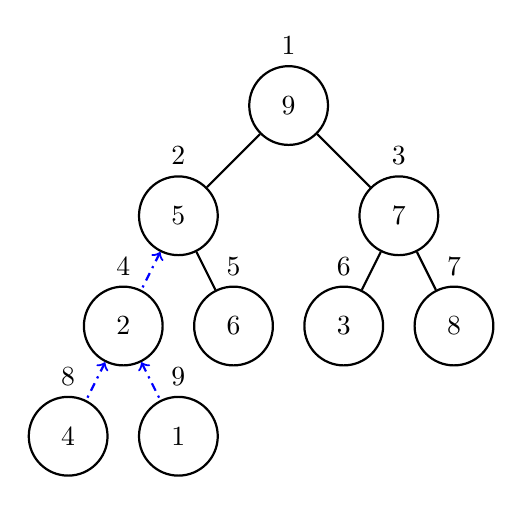
\begin{tikzpicture}[thick, scale=0.7]
        \node[label={1},circle,draw,minimum size=1cm]
        (1) at (0,0) {$9$};
        \node[label={2},circle,draw,minimum size=1cm]
        (2) at (-2,-2) {$5$};
        \node[label={3},circle,draw,minimum size=1cm]
        (3) at (2,-2) {$7$};
        \node[label={4},circle,draw,minimum size=1cm]
        (4) at (-3,-4) {$2$};
        \node[label={5},circle,draw,minimum size=1cm]
        (5) at (-1,-4) {$6$};
        \node[label={6},circle,draw,minimum size=1cm]
        (6) at (1,-4) {$3$};
        \node[label={7},circle,draw,minimum size=1cm]
        (7) at (3,-4) {$8$};
        \node[label={8},circle,draw,minimum size=1cm]
        (8) at (-4,-6) {$4$};
        \node[label={9},circle,draw,minimum size=1cm]
        (9) at (-2,-6) {$1$};

        \tikzstyle{cert}=[<-, dashdotted, blue, thick]
        \draw[thick] (1) -- (2);
        \draw[thick] (1) -- (3);
        \draw[cert] (2) -- (4);
        \draw[thick] (2) -- (5);
        \draw[thick] (3) -- (6);
        \draw[thick] (3) -- (7);
        \draw[cert] (4) -- (8);
        \draw[cert] (4) -- (9);
    \end{tikzpicture}
    \caption[Exemplo certificados do heap cinético após operação \textsc{change}]{Após a mudança de
    velocidade do elemento 2, que se encontra em \heap[$4$], os certificados
    \cert[$4$], \cert[$8$] e \cert[$9$] foram atualizados.}
    \label{fig:predeventheap}
\end{figure}

\subsection{Análise de desempenho}\label{subsec:analise-de-desempenho}

A lista ordenada cinética é uma estrutura \textit{responsiva}, pois o custo de
processar um certificado é exatamente o custo da rotina \textsc{event}, que é $O(\lg{n})$ pois a
rotina \textsc{update} consome $O(\lg{n})$ para atualizar a fila de prioridade dos certificados.

A lista ordenada cinética é uma estrutura \textit{eficiente}, pois todos os eventos
processados são eventos \textit{externos}, isto é, todo vencimento de
certificado representa a troca de ordem entre dois elementos na lista, que é uma
mudança na descrição combinatória do problema.

A lista ordenada cinética é uma estrutura \textit{compacta}, pois como cada
certificado está associado à relação de ordem entre um elemento e seu
predecessor, teremos no máximo $n-1$ certificados na fila de prioridades num
determinado instante.

A lista ordenada cinética é uma estrutura \textit{local}, pois cada elemento
está relacionado a no máximo dois certificados, o certificado entre ele e o
seu predecessor e o certificado entre o seu sucessor e ele.

%!TeX root=./ordenacao.tex

\section{Árvore binária balanceada de busca} \label{abb}

Manter um vetor ordenado é uma boa maneira de resolver o problema da
lista ordenada cinética dando suporte às operações
\textsc{advance}$(t)$, \textsc{change}$(j,v)$ e
\textsc{query\_kth}$(i)$. Poderíamos também querer dar suporte, além
das operações citadas, às seguintes operações:

\begin{itemize}
    \item \textsc{insert}$(v, x_t) \rightarrow$ insere um
    elemento com velocidade $v$ e valor $x_t$ no instante \now;
    \item \textsc{delete}$(i) \rightarrow$ remove o elemento
    $i$ no instante \now.
\end{itemize}

Para inserir um elemento no vetor ordenado, antes teríamos de
encontrar a posição que este deveria ocupar no vetor. Digamos que
seja a posição $j$. Após encontrar a posição, movemos todos os
elementos, a partir da posição $j$, uma posição à frente e colocamos
o elemento na posição~$j$. Após isso, os certificados de $j$~até~$n
- 1$ devem ser atualizados, pois esses elementos mudaram de posição
no vetor, e um novo certificado será criado, o $n$-ésimo
certificado, o total de elementos $n$ deve ser mudado para $n + 1$.
O novo certificado também deve ser inserido na fila com prioridades.

Só a operação de inserir um novo elemento no vetor já pode se tornar
pouco eficiente com uma grande quantidade de elementos sendo
inseridos no começo do vetor, consumindo tempo linear por inserção.
Como a remoção de um elemento no vetor ordenado envolve uma
sequência parecida de operações, da mesma maneira se torna pouco
eficiente, também consumindo tempo linear no pior caso.

Dessa forma, apesar da lista ordenada cinética implementada
manipulando um vetor ser uma estrutura eficiente para a operação
\textsc{query\_kth}$(i)$, com um consumo de tempo constante, o
consumo de tempo para as operações \textsc{insert}$(v, x_t)$ e
\textsc{delete}$(i)$ é, no pior caso, proporcional ao número de
elementos, o que pode ser ruim para uma grande quantidade de
elementos, inserções e remoções.

Podemos equilibrar o consumo de tempo das operações
\textsc{query\_kth}$(i)$, \textsc{insert}$(v, x_t)$ e
\textsc{delete}$(i)$ em tempo logarítmico no número de elementos,
usando uma ABBB (árvore binária balanceada de busca). Os pontos
serão armazenados na ABBB tendo o seu valor no instante \now~como
chave.

Além da ABBB, para garantirmos a eficiência das operações
\textsc{event}, \textsc{change}, \textsc{insert} e \textsc{delete},
cada elemento terá um apontador para o seu predecessor e um
apontador para o seu sucessor, formando uma lista duplamente ligada
ordenada pelo valor do elemento no instante \now; veja a Figura
\ref{fig:abb:exemplo}.

\begin{figure}[H]
    \centering
    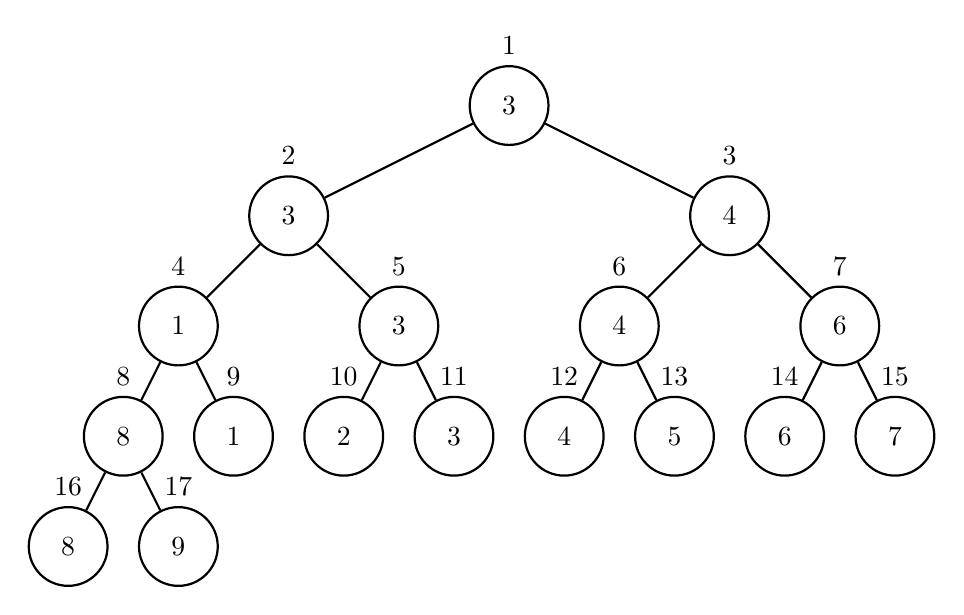
\begin{tikzpicture}[thick, scale=0.7]
        \node[label={1},circle,draw,minimum size=1cm]
        (1) at (0,0) {$3$};
        \node[label={2},circle,draw,minimum size=1cm]
        (2) at (-4,-2) {$3$};
        \node[label={3},circle,draw,minimum size=1cm]
        (3) at (4,-2) {$4$};
        \node[label={4},circle,draw,minimum size=1cm]
        (4) at (-6,-4) {$1$};
        \node[label={5},circle,draw,minimum size=1cm]
        (5) at (-2,-4) {$3$};
        \node[label={6},circle,draw,minimum size=1cm]
        (6) at (2,-4) {$4$};
        \node[label={7},circle,draw,minimum size=1cm]
        (7) at (6,-4) {$6$};
        \node[label={8},circle,draw,minimum size=1cm]
        (8) at (-7,-6) {$8$};
        \node[label={9},circle,draw,minimum size=1cm]
        (9) at (-5,-6) {$1$};
        \node[label={10},circle,draw,minimum size=1cm]
        (10) at (-3,-6) {$2$};
        \node[label={11},circle,draw,minimum size=1cm]
        (11) at (-1,-6) {$3$};
        \node[label={12},circle,draw,minimum size=1cm]
        (12) at (1,-6) {$4$};
        \node[label={13},circle,draw,minimum size=1cm]
        (13) at (3,-6) {$5$};
        \node[label={14},circle,draw,minimum size=1cm]
        (14) at (5,-6) {$6$};
        \node[label={15},circle,draw,minimum size=1cm]
        (15) at (7,-6) {$7$};
        \node[label={16},circle,draw,minimum size=1cm]
        (16) at (-8,-8) {$8$};
        \node[label={17},circle,draw,minimum size=1cm]
        (17) at (-6,-8) {$9$};

        \draw[thick] (1) -- (2);
        \draw[thick] (2) -- (4);
        \draw[thick] (4) -- (8);
        \draw[thick] (4) -- (9);
        \draw[thick] (8) -- (16);
        \draw[thick] (8) -- (17);
        \draw[thick] (2) -- (5);
        \draw[thick] (5) -- (10);
        \draw[thick] (5) -- (11);
        \draw[thick] (1) -- (3);
        \draw[thick] (3) -- (6);
        \draw[thick] (3) -- (7);
        \draw[thick] (6) -- (12);
        \draw[thick] (6) -- (13);
        \draw[thick] (7) -- (14);
        \draw[thick] (7) -- (15);
    \end{tikzpicture}
    \caption[Representação da estrutura torneio]{Torneio com $9$
        elementos em que $3$ é o elemento com valor máximo.}
    \label{fig:torneio:exemplo}
\end{figure}

No que diz respeito aos certificados, antes um certificado estava
associado a uma posição e, no vetor, ao inserirmos um elemento em
uma determinada posição, teríamos que deslocar % que atualizar
todos os certificados conseguintes àquela posição. Agora, para que
consigamos alterar apenas uma quantidade constante de certificados
após uma inserção, os certificados não estarão mais associados a uma
posição e sim aos elementos.

O certificado $i$ se refere à relação estabelecida entre o elemento
$i$ e seu predecessor e consiste no instante de tempo em que o
elemento $i$ deixará de ter um valor maior que o valor do seu
predecessor, se esse instante for maior que o instante atual. Do
contrário, o certificado consiste em $+\infty$. Se o elemento $i$
não possui predecessor, então o certificado também consiste em
$+\infty$. Veja a Figura \ref{fig:abb:cert}.

Esses $n$ certificados também serão colocados em uma fila com
prioridades, com o prazo de validade determinando a prioridade.
A fila com prioridades agora também deverá suportar operações
como a inserção e remoção de certificados.

\begin{figure}[htb]
    \centering
    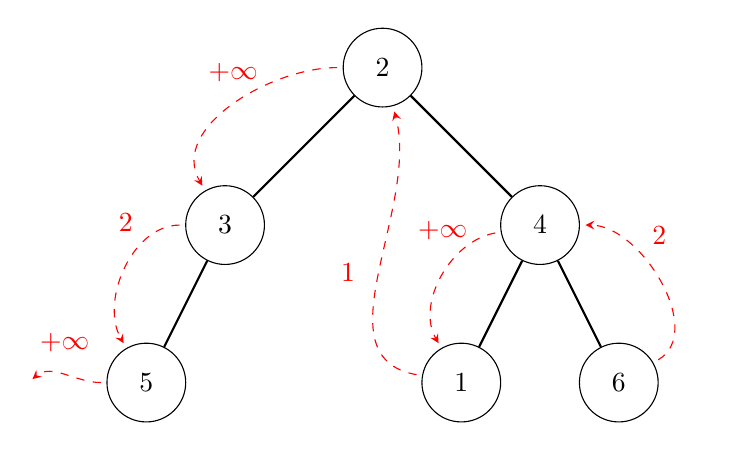
\begin{tikzpicture}[baseline=-2.25cm]
        \node[circle,draw,minimum size=1cm] (1) at (0,0)  {$2$};
        \node[circle,draw,minimum size=1cm] (2) at (-2,-2){$3$};
        \node[circle,draw,minimum size=1cm] (3) at (2,-2) {$4$};
        \node[circle,draw,minimum size=1cm] (4) at (-3,-4){$5$};
        \node[circle,draw,minimum size=1cm] (5) at (1,-4) {$1$};
        \node[circle,draw,minimum size=1cm] (6) at (3,-4) {$6$};
        \tikzstyle{filho}=[thick]
        \tikzstyle{pred}=[->, shorten >= 2pt, shorten <= 2pt,
        dashed, >=stealth, red]
        \tikzstyle{sucessor}=[->, shorten >= 2pt, shorten <= 2pt,
        dotted, >=stealth, line width=0.35mm]
        \draw[filho] (1) -- (2);
        \draw[filho] (1) -- (3);
        \draw[filho] (2) -- (4);
        \draw[filho] (3) -- (5);
        \draw[filho] (3) -- (6);
        \draw[pred] (6) edge[out=30,in=0] node[above=10pt, red] {$2$} (3);
        % \node[red] at (4,-3) {$2$};
        \draw[pred] (3) edge[out=190,in=120]
        node[above=10pt, red] {$+\infty$} (5);
        \draw[pred] (5) edge[out=170,in=285]
        node[left=5pt, red] {$1$} (1);
        \draw[pred] (1) edge[out=180,in=120]
        node[above=5pt, red] {$+\infty$} (2);
        \draw[pred] (2) edge[out=180,in=120]
        node[above=10pt, red] {$2$} (4);
        \draw[pred] (4) edge[out=180,in=40]
        node[above=5pt, red] {$+\infty$} (-4.5, -4);
    \end{tikzpicture}
    \qquad
    \qquad
    \qquad
    \begin{tabular}{|c|c|c|c|}
        \hline
        $i$ & $x_0$ & $v$   & $\cert[i]$ \\
        \hline
        $1$ & $6$   & $2$   & $1$        \\

        $2$ & $3$   & $5$   & $+\infty$  \\

        $3$ & $2$   & $1$   & $2$        \\

        $4$ & $7$   & $4$   & $+\infty$  \\

        $5$ & $-2$  & $3$   & $+\infty$  \\

        $6$ & $14$  & $0.5$ & $2$        \\
        \hline
    \end{tabular}
    \caption[Representação dos certificados da ABB]{Certificados
    representados pelas setas vermelhas tracejadas. O
    elemento $5$ é o último da lista e o seu certificado vale $+\infty$.}
    \label{fig:abb:cert}
\end{figure}

Para descrever as implementações das operações, vamos
estabelecer os nomes dos objetos, variáveis e rotinas
auxiliares utilizados:
\begin{enumerate}
    \item $n$: número de elementos no instante \now;
    \item \no: objeto que compõe a árvore binária balanceada
            de busca, com atributos:
    \begin{enumerate}
        \item \esq$:$ aponta para a raiz da subárvore
        esquerda do nó;
        \item \dir$:$ aponta para a raiz da subárvore
        direita do nó;
        \item \textit{key}$:$ aponta para um elemento;
        \item \children$:$ quantidade de nós que a subárvore
        enraizada neste nó possui. Este atributo será importante
        para a operação \textsc{query\_kth}$(i)$;
    \end{enumerate}
    \item \raiz: nó que é a raiz da árvore binária balanceada de
                busca;
    \item \elemento: objeto com os seguintes atributos:
    \begin{enumerate}
        \item \id: vem de \textit{identifier} e é o atributo
        para identificar o objeto. Assim, daqui
        em diante, usaremos elemento $i$ para nos
        referirmos ao elemento cujo \id~é $i$;
        \item \speed: velocidade do elemento;
        \item \initv: valor que o elemento possuía no
        instante~$t = 0$;
        \item \nex: apontador para o elemento imediatamente
        posterior a este na coleção, no instante \now. O
        elemento imediatamente posterior a $i$ é aquele
        que possui o menor valor dentre a coleção de
        elementos que possuem valor maior que o elemento
        $i$;
        \item \prev: apontador para o elemento imediatamente
        anterior a este na coleção, no instante \now;
        \item \pqpos: vem de \textit{priority queue position} e
        aponta para a posição do certificado associado
        ao elemento na fila com prioridades;
        \item \cert: vem de \textit{certificate} e é o prazo de
        validade do certificado entre este elemento e o elemento
        apontado por \prev; se \prev~não aponta para ninguém,
        \cert~vale $+\infty$;
        \item \no: apontador para o nó da árvore binária de busca em
        que o elemento se encontra;
    \end{enumerate}
    \item \Q: fila com prioridades que contém os elementos; o
    elemento com certificado de menor valor estará à frente da fila;

    \item \textsc{insertKey}$(\text{\raiz},e)\rightarrow$ insere
    $e$, um elemento, na árvore binária balanceada de busca com raiz
    \raiz~e retorna a, possivelmente nova, raiz da árvore. No
    processo também atualiza a lista ligada de elementos;

    \item \textsc{deleteKey}$(\text{\raiz},e)\rightarrow$ remove
    $e$, um elemento, da árvore binária balanceada de busca com raiz
    \raiz~e retorna a, possivelmente nova, raiz da árvore. No
    processo também atualiza a lista ligada de elementos.

\end{enumerate}
Para a implementação das operações \textsc{change}$(j, v)$ e
\textsc{delete}$(i)$, precisamos de alguma maneira recuperar um
elemento baseado no seu \id. Para tal, podemos utilizar uma tabela
de símbolos, implementada por uma árvore binária balanceada de busca
ou uma tabela de dispersão. A seguir~estão três operações que nos
ajudarão a recuperar os elementos:

\begin{enumerate}
    \item \textsc{getObject}$(i)\rightarrow$ retorna o elemento $i$;
    \item \textsc{insertObject}$(e) \rightarrow$ insere $e$,
    que é um elemento, na estrutura;
    \item \textsc{deleteObject}$(e) \rightarrow$ remove $e$,
    que é um elemento, da estrutura.
\end{enumerate}

Para permitir a inserção e remoção de certificados, a interface da
fila com prioridades será reformulada, contando com duas operações
extras:

\begin{enumerate}
    \item \textsc{insertPQ}$(Q, e) \rightarrow$ insere $(e, t)$
    na fila com prioridades $Q$;
    \item \textsc{deletePQ}$(Q, e) \rightarrow$ remove $e$
    da fila com prioridades $Q$;
    \item \textsc{updatePQ}$(Q,e,t) \rightarrow$ muda o prazo de
    validade do certificado de $e$ para $t$ e atualiza a fila com
    prioridades $Q$;
    \item \textsc{minPQ}$(Q) \rightarrow$ devolve o elemento com o
    certificado de menor prazo de validade da fila com prioridades
    $Q$.
\end{enumerate}

A operação \textsc{updatePQ}$(Q,e,t)$ pode ser implementada de modo
a consumir tempo logarítmico no número de elementos em $Q$ graças ao
atributo \pqpos~dos elementos.

Um evento está associado a um par $(e, t)$ que corresponde ao
certificado do elemento $e$ que expira no instante $t$. O tratamento
do evento correspondente a esse par $(e, t)$ consiste em trocar de
lugar o elemento $e$ e seu predecessor, digamos $e'$, na árvore
binária de busca e na lista ligada, e recalcular o prazo de validade
de até três certificados:

\begin{itemize}
    \item do certificado de $e$;
    \item do certificado de $e'$;
    \item do certificado do novo sucessor de $e'$, caso não seja \textsc{null}.
\end{itemize}

Na implementação da operação \textsc{event}, no Algoritmo
\ref{abb:evento}, utilizaremos a rotina $\textsc{update}(e)$, no
Algoritmo \ref{abb:update}, que calcula o novo prazo de validade $t$
do certificado do elemento $e$, e chama a
rotina~$\textsc{updatePQ}(Q, e, t)$. A função $\textsc{swap}(e_1,
e_2)$ troca a posição de $e_1$ e $e_2$ na árvore binária balanceada
de busca e na lista ligada e a função \Call{expire}{$e,e'$} calcula
a validade do certificado entre os elementos $e$ e $e'$; se $e'$ é
\textsc{null} retorna $+\infty$.

\begin{algorithm}
    \caption{Função \textsc{update}.} \label{lista:update}
\begin{algorithmic}[1]
    \Function{update}{$i$}
        \If{$1 \leq i < n$}
            \State $t \leftarrow $ \Call{expire}{$i,i+1$}
            \State \Call{updatePQ}{$Q,i,t$}
        \EndIf
    \EndFunction
\end{algorithmic}
\end{algorithm}

\begin{algorithm}
    \caption{Função \textsc{event}.} \label{torneioi:evento}
    \begin{algorithmic}[1]
        \Function{event}{\nnull}
            \State $e \leftarrow  $ \Call{minPQ}{$Q$}
            \While{$e.\cert$ = \now}
                \State $j \leftarrow e.\lastmatch$
                \State $k \leftarrow 2\cdot \floor{\frac{j}{2}}
                + ((j + 1)\mod2)$ \Comment{adversário}
                \While{$j > 1$ \AND \Call{compare}{$j, k$}}
                    \State \torneio[$\floor{\frac{j}{2}}$]
                    $\leftarrow~$\torneio[$j$]
                    \State $\torneio[k].\lastmatch$ $\leftarrow k$
                    \State \Call{update}{$\torneio[k]$}
                    \State $j \leftarrow \floor{\frac{j}{2}}$
                    \State $k \leftarrow 2\cdot \floor{\frac{j}{2}}
                    + ((j + 1)\mod2)$ \Comment{adversário}
                \EndWhile
                \State $\torneio[j].\lastmatch \leftarrow j$
                \State \Call{update}{$\torneio[j]$}
                \State $e \leftarrow  $ \Call{minPQ}{$Q$}
            \EndWhile
        % \LineComment{swapHeap$(i, \floor{\frac{i}{2}})$ troca \heap[$i$] por \heap$\left[\floor{\frac{i}{2}}\right]$}
        \EndFunction
        \LineComment{\Call{compare}{$i, j$} retorna se o valor
        de $i$ é maior que o valor de $j$.}
    \end{algorithmic}
\end{algorithm}

\begin{figure}
    \centering
    \begin{tikzpicture}[thick, scale=0.8]
        \node[label={1},circle,draw,minimum size=1cm]
            (1) at (0,0) {$3$};
        \node[label={2},circle,draw,minimum size=1cm]
            (2) at (-4,-2) {$3$};
        \node[label={3},circle,draw,minimum size=1cm]
            (3) at (4,-2) {$4$};
        \node[label={4},circle,draw,minimum size=1cm]
            (4) at (-6,-4) {$1$};
        \node[label={5},circle,draw,minimum size=1cm]
            (5) at (-2,-4) {$3$};
        \node[label={6},circle,draw,minimum size=1cm]
            (6) at (2,-4) {$4$};
        \node[label={7},circle,draw,minimum size=1cm]
            (7) at (6,-4) {$6$};
        \node[label={8},circle,draw,minimum size=1cm]
            (8) at (-7,-6) {$8$};
        \node[label={9},circle,draw,minimum size=1cm]
            (9) at (-5,-6) {$1$};
        \node[label={10},circle,draw,minimum size=1cm]
            (10) at (-3,-6) {$2$};
        \node[label={11},circle,draw,minimum size=1cm]
            (11) at (-1,-6) {$3$};
        \node[label={12},circle,draw,minimum size=1cm]
            (12) at (1,-6) {$4$};
        \node[label={13},circle,draw,minimum size=1cm]
            (13) at (3,-6) {$5$};
        \node[label={14},circle,draw,minimum size=1cm]
            (14) at (5,-6) {$6$};
        \node[label={15},circle,draw,minimum size=1cm]
            (15) at (7,-6) {$7$};
        \node[label={16},circle,draw,minimum size=1cm]
            (16) at (-8,-8) {$8$};
        \node[label={17},circle,draw,minimum size=1cm]
            (17) at (-6,-8) {$9$};

        \draw[thick] (1) -- (2);
        \draw[<-,line width=\thickness, red] (2) -- (4);
        \draw[<-,thick, dashed, red] (4) -- (8);
        \draw[thick] (4) -- (9);
        \draw[thick] (8) -- (16);
        \draw[<-,line width=\thickness, red] (8) -- (17);
        \draw[thick] (2) -- (5);
        \draw[<-,line width=\thickness, red] (5) -- (10);
        \draw[thick] (5) -- (11);
        \draw[<-,line width=\thickness, red] (1) -- (3);
        \draw[thick] (3) -- (6);
        \draw[<-,line width=\thickness, red] (3) -- (7);
        \draw[thick] (6) -- (12);
        \draw[<-,line width=\thickness, red] (6) -- (13);
        \draw[thick] (7) -- (14);
        \draw[<-,line width=\thickness, red] (7) -- (15);
    \end{tikzpicture}
    \caption[Representação de certificado expirado]{cert[$8$] expirou.}
    \label{fig:torneio:evento}
\end{figure}

\begin{figure}[H]
    \centering
    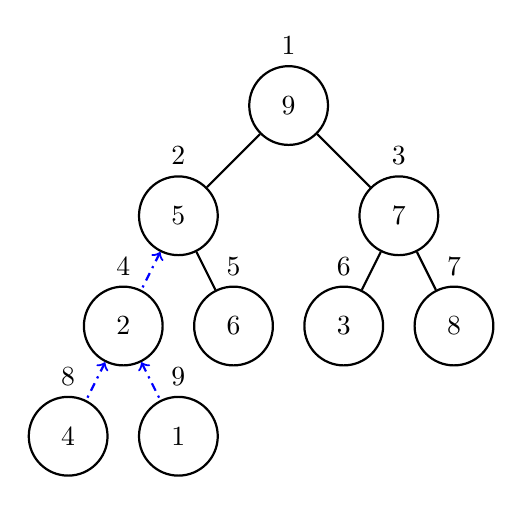
\begin{tikzpicture}[thick, scale=0.7]
        \node[label={1},circle,draw,minimum size=1cm]
        (1) at (0,0) {$9$};
        \node[label={2},circle,draw,minimum size=1cm]
        (2) at (-2,-2) {$5$};
        \node[label={3},circle,draw,minimum size=1cm]
        (3) at (2,-2) {$7$};
        \node[label={4},circle,draw,minimum size=1cm]
        (4) at (-3,-4) {$2$};
        \node[label={5},circle,draw,minimum size=1cm]
        (5) at (-1,-4) {$6$};
        \node[label={6},circle,draw,minimum size=1cm]
        (6) at (1,-4) {$3$};
        \node[label={7},circle,draw,minimum size=1cm]
        (7) at (3,-4) {$8$};
        \node[label={8},circle,draw,minimum size=1cm]
        (8) at (-4,-6) {$4$};
        \node[label={9},circle,draw,minimum size=1cm]
        (9) at (-2,-6) {$1$};

        \tikzstyle{cert}=[<-, dashdotted, blue, thick]
        \draw[thick] (1) -- (2);
        \draw[thick] (1) -- (3);
        \draw[cert] (2) -- (4);
        \draw[thick] (2) -- (5);
        \draw[thick] (3) -- (6);
        \draw[thick] (3) -- (7);
        \draw[cert] (4) -- (8);
        \draw[cert] (4) -- (9);
    \end{tikzpicture}
    \caption[Exemplo certificados do heap cinético após operação \textsc{change}]{Após a mudança de
    velocidade do elemento 2, que se encontra em \heap[$4$], os certificados
    \cert[$4$], \cert[$8$] e \cert[$9$] foram atualizados.}
    \label{fig:predeventheap}
\end{figure}

A operação \textsc{query\_kth}$(i)$ consiste em devolver o $i$-ésimo
maior elemento da lista ligada, ou seja, o $i$-ésimo da direita para
a esquerda, pois a árvore está em ordem crescente da esquerda para a
direita. Para tal, percorreremos a árvore binária balanceada de
busca utilizando o atributo $\children$ para, a cada iteração,
decidir em qual subárvore o $i$-ésimo está, ajustando $i$ quando
necessário. O Algoritmo \ref{abb:query} implementa esta operação e a
Figura \ref{fig:abb:queryexecution} simula a execução em um exemplo.
A rotina auxiliar \textsc{rsize}$(r)$ devolve o valor de
$r.right.\textit{size}$ caso este seja não nulo, caso contrário
devolve $0$.


% Estando em um determinado nó \no~da árvore, sabemos que todos os nós
% na subárvore direita tem valor maior que o nó atual e que os nós da
% subárvore esquerda. Portanto, se $i \leq node.right.\children$, a
% nossa resposta com certeza está na subárvore direita do nó. Caso
% contrário temos duas opções: \no~é a resposta ou a resposta está na
% subárvore esquerda. Para checar se \no~é a resposta, devemos
% perceber que \no~tem valor maior que os nós de sua subárvore
% esquerda, então se $i = node.right.\children + 1$, \no~é a resposta.
% Se $i > node.right.\children + 1$, então a nossa resposta está na
% subárvore esquerda e queremos o $[i - (node.right.\children +
% 1)]$-ésimo elemento da subárvore esquerda. Podemos repetir esse
% processo até encontrar a nossa resposta. O Algoritmo \ref{abb:query}
% utiliza a rotina auxiliar \textsc{rsize}$(r)$, que devolve o valor
% de \textit{size} de $r.right$ caso este seja não nulo, caso
% contrário devolve $0$.
% Se, dada uma raiz, soubermos a quantidade de filhos
% direitos,~\raiz$.rsize$, comparamos com o valor de $i$ e podemos
% ter três conclusões: se~$i > root.rsize$, significa que o
% $i$-ésimo elemento com certeza não está na subárvore direita, pois
% todos elementos da subárvore direita estão a frente de \raiz~e da
% subárvore esquerda. Nesse caso, calculamos $i - root.rsize$, se
% esse valor é igual a $1$, então \raiz~é o $i-ésimo$ elemento da
% coleção, pois \raiz~é o próximo elemento após todos elementos na
% subárvore direita. Se $root.rsize - i \neq 1$, então devemos

\begin{algorithm}
    \caption{Função \textsc{query\_kth}.} \label{lista:query}
\begin{algorithmic}[1]
    \Function{query\_kth}{$i$}
        \If{$1 \leq i \leq n$}
            \State \Return \sorted[$i$]
        \EndIf
        \State \Return $-1$
    \EndFunction
\end{algorithmic}
\end{algorithm}

\begin{figure}[H]
    \centering
    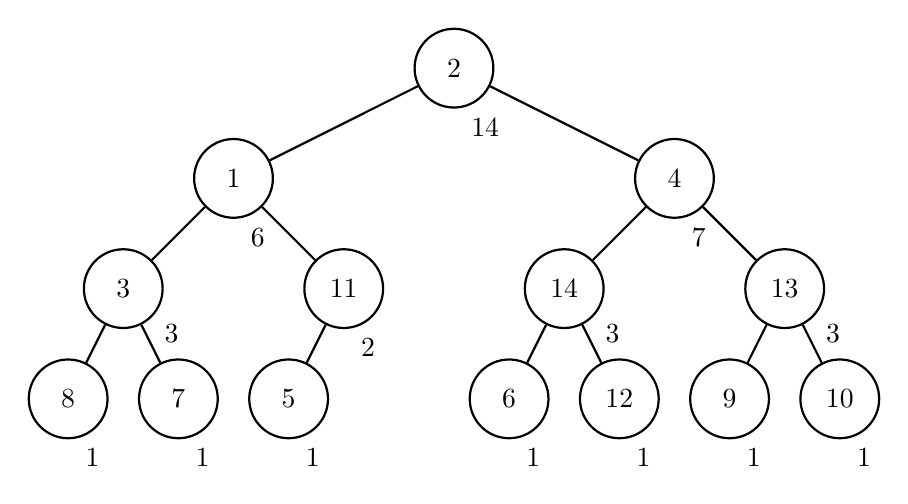
\begin{tikzpicture}[thick,scale=0.7]
        \node[label=280:{14},circle,draw,minimum size=1cm]
        (1) at (0,0) {$2$};
        \node[label=280:{6},circle,draw,minimum size=1cm]
        (2) at (-4,-2) {$1$};
        \node[label=280:{7},circle,draw,minimum size=1cm]
        (3) at (4,-2) {$4$};
        \node[label=320:{3},circle,draw,minimum size=1cm]
        (4) at (-6,-4) {$3$};
        \node[label=280:{2},circle,draw,minimum size=1cm]
        (5) at (-2,-4) {$11$};
        \node[label=320:{3},circle,draw,minimum size=1cm]
        (6) at (2,-4) {$14$};
        \node[label=320:{3},circle,draw,minimum size=1cm]
        (7) at (6,-4) {$13$};
        \node[label=280:{1},circle,draw,minimum size=1cm]
        (8) at (-7,-6) {$8$};
        \node[label=280:{1},circle,draw,minimum size=1cm]
        (9) at (-5,-6) {$7$};
        \node[label=280:{1},circle,draw,minimum size=1cm]
        (10) at (-3,-6) {$5$};
        % \node[label={11},circle,draw,minimum size=1cm] (11) at (-1,-6) {$3$};
        \node[label=280:{1},circle,draw,minimum size=1cm]
        (12) at (1,-6) {$6$};
        \node[label=280:{1},circle,draw,minimum size=1cm]
        (13) at (3,-6) {$12$};
        \node[label=280:{1},circle,draw,minimum size=1cm]
        (14) at (5,-6) {$9$};
        \node[label=280:{1},circle,draw,minimum size=1cm]
        (15) at (7,-6) {$10$};

        \draw[thick] (1) -- (2);
        \draw[thick] (2) -- (4);
        \draw[thick] (4) -- (8);
        \draw[thick] (4) -- (9);
        \draw[thick] (2) -- (5);
        \draw[thick] (5) -- (10);
        % \draw[thick] (5) -- (11);
        \draw[thick] (1) -- (3);
        \draw[thick] (3) -- (6);
        \draw[thick] (3) -- (7);
        \draw[thick] (6) -- (12);
        \draw[thick] (6) -- (13);
        \draw[thick] (7) -- (14);
        \draw[thick] (7) -- (15);
    \end{tikzpicture}
    \caption[Exemplo de árvore binária de busca com campo \children]{Exemplo de ABB com campo \children.}
    \label{fig:abb:query}
\end{figure}

\begin{figure}[H]
    \centering
    \begin{tikzpicture}[thick,scale=0.7]
        \tikzstyle{triangle} = [regular polygon, regular polygon sides=3]
        \node[
        label=280:{14},
        label=80:{$i = 7 \leq 7$},
        very thick,
        circle,
        draw,
        minimum size=1cm]
        (1) at (0,0) {$2$};
        \node[label=280:{6},triangle,draw,minimum size=1cm]
        (2) at (-4,-2) {};

        \node[label=280:{7},
        label=80:{$i = 7 > 3$},
        very thick,
        circle,draw,minimum size=1cm]
        (3) at (4,-2) {$4$};
        % \node[label=320:{3},circle,draw,minimum size=1cm]
        %     (4) at (-6,-4) {$3$};
        % \node[label=280:{2},circle,draw,minimum size=1cm]
        %     (5) at (-2,-4) {$11$};
        \node[label=320:{3},
        label=120:{$i = 3 > 1$},
        very thick,
        circle,draw,minimum size=1cm]
        (6) at (2,-4) {$14$};

        \node[label=320:{3},triangle,draw,minimum size=1cm]
        (7) at (6,-4) {};
        % \node[label=280:{1},circle,draw,minimum size=1cm]
        %     (8) at (-7,-6) {$8$};
        % \node[label=280:{1},circle,draw,minimum size=1cm]
        %     (9) at (-5,-6) {$7$};
        % \node[label=280:{1},circle,draw,minimum size=1cm]
        %     (10) at (-3,-6) {$5$};
        % \node[label={11},circle,draw,minimum size=1cm] (11) at (-1,-6) {$3$};
        \node[label=280:{1},
        label=120:{$i = 1 = 0 + 1$},
        very thick,
        circle,draw,minimum size=1cm]
        (12) at (1,-6) {$6$};

        \node[label=280:{1},triangle,draw,minimum size=1cm]
        (13) at (3,-6) {};
        % \node[label=280:{1},circle,draw,minimum size=1cm]
        %     (14) at (5,-6) {$9$};
        % \node[label=280:{1},circle,draw,minimum size=1cm]
        %     (15) at (7,-6) {$10$};

        \draw[thick] (1) -- (2);
        % \draw[thick] (2) -- (4);
        % \draw[thick] (4) -- (8);
        % \draw[thick] (4) -- (9);
        % \draw[thick] (2) -- (5);
        % \draw[thick] (5) -- (10);
        % \draw[thick] (5) -- (11);
        \draw[very thick] (1) -- node[above, sloped] {$i = 7$} (3);
        \draw[very thick] (3) -- node[above, sloped] {$i = 3$} (6);
        \draw[thick] (3) -- (7);
        \draw[very thick] (6) -- (12);% node[above, sloped] {$i = 1$} (12);
        \draw[thick] (6) -- (13);
        % \draw[thick] (7) -- (14);
        % \draw[thick] (7) -- (15);
    \end{tikzpicture}
    \caption[Exemplo de busca pelo $i$-ésimo]{Exemplo de busca pelo
    $7^\circ$ elemento da direita para a esquerda na árvore da
    Figura \ref{fig:abb:query}.}
    \label{fig:abb:queryexecution}
\end{figure}

A operação \textsc{change}$(j, v)$, como implementada no Algoritmo
\ref{abb:change}, consiste em recuperar o elemento $e$ com
identificador $j$, alterar seu atributo \initv~para $x_0 +
(\mathit{speed} - v)\cdot now$, \textit{speed} para \textit{v} e
recalcular os eventuais certificados de que $j$ participa, que
seriam $e.cert$ e $e.next.cert$, se $e.next$ existe. A Figura
\ref{fig:abb:change} ilustra um exemplo com os elementos afetados.

\begin{algorithm}
    \caption{Função \textsc{change}.} \label{torneioi:change}
    \begin{algorithmic}[1]
        \Function{change}{$j, v$}
            \State $e \leftarrow$ \Call{getObject}{$j$}
            \State $e.x_0 \leftarrow e.x_0+~(e.\speed -~v)~\cdot~\now$;
            \State $e.\speed \leftarrow v$
            \State $i \leftarrow e.\lastmatch$
            \State \Call{update}{$e$}
            \While{$i < n$}
                \If{$\torneio[i] = \torneio[2i]$}
                    \State $i \leftarrow 2i$
                \Else
                    \State $i \leftarrow 2i + 1$
                \EndIf
                \State $k \leftarrow 2\cdot \floor{\frac{i}{2}}
                + ((i + 1)\mod2)$ \Comment{adversário}
                \State \Call{update}{$\torneio[k]$}
            \EndWhile
        \EndFunction
    \end{algorithmic}
\end{algorithm}

\begin{algorithm}
    \caption{Função \textsc{change}.} \label{torneioi:change}
    \begin{algorithmic}[1]
        \Function{change}{$j, v$}
            \State $e \leftarrow$ \Call{getObject}{$j$}
            \State $e.x_0 \leftarrow e.x_0+~(e.\speed -~v)~\cdot~\now$;
            \State $e.\speed \leftarrow v$
            \State $i \leftarrow e.\lastmatch$
            \State \Call{update}{$e$}
            \While{$i < n$}
                \If{$\torneio[i] = \torneio[2i]$}
                    \State $i \leftarrow 2i$
                \Else
                    \State $i \leftarrow 2i + 1$
                \EndIf
                \State $k \leftarrow 2\cdot \floor{\frac{i}{2}}
                + ((i + 1)\mod2)$ \Comment{adversário}
                \State \Call{update}{$\torneio[k]$}
            \EndWhile
        \EndFunction
    \end{algorithmic}
\end{algorithm}

\begin{figure}[H]
    \centering
    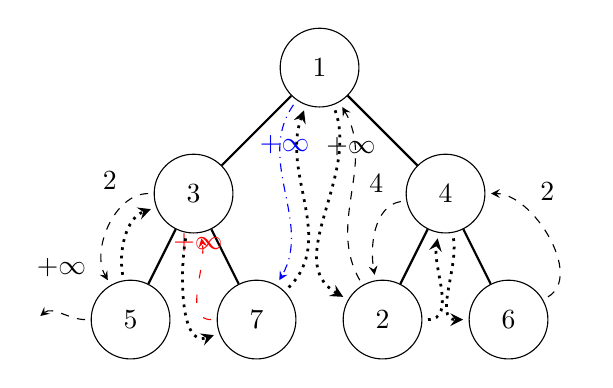
\begin{tikzpicture}[baseline=-2cm,scale=0.8]
        \node[circle,draw,minimum size=1cm] (1) at (0,0)  {$1$};
        \node[circle,draw,minimum size=1cm] (2) at (-2,-2){$3$};
        \node[circle,draw,minimum size=1cm] (3) at (2,-2) {$4$};
        \node[circle,draw,minimum size=1cm] (4) at (-3,-4){$5$};
        \node[circle,draw,minimum size=1cm] (5) at (1,-4) {$2$};
        \node[circle,draw,minimum size=1cm] (6) at (3,-4) {$6$};
        \node[circle,draw,minimum size=1cm] (7) at (-1,-4){$7$};
        % \node[label={7},circle,draw,minimum size=1cm] (7) at (3,-4) {$8$};
        % \node[label={9},circle,draw,minimum size=1cm] (9) at (-2,-6) {$1$};
        \tikzstyle{filho}=[thick]
        \tikzstyle{pred}=[->, shorten >= 2pt, shorten <= 2pt,
        dashed, >=stealth]
        \tikzstyle{sucessor}=[->, shorten >= 2pt, shorten <= 2pt,
        dotted, >=stealth, line width=0.35mm]
        % \tikzstyle{p4}=[->, shorten >= 2pt, shorten <= 2pt, dotted, >=stealth]
        \draw[filho] (1) -- (2);
        \draw[filho] (1) -- (3);
        \draw[filho] (2) -- (4);
        \draw[filho] (2) -- (7);
        \draw[filho] (3) -- (5);
        \draw[filho] (3) -- (6);
        \draw[pred] (6) edge[out=30,in=0]
        node[above=10pt] {$2$} (3);
        \draw[sucessor] (3) edge[out=280,in=180] (6);
        \draw[pred] (3) edge[out=190,in=100]
        node[above=10pt] {$4$} (5);
        \draw[sucessor] (5) edge[out=0,in=260] (3);
        \draw[pred] (5) edge[out=120,in=300]
        node[above=10pt] {$+\infty$} (1);
        \draw[sucessor] (1) edge[out=290,in=150] (5);
        \draw[pred, loosely dashed, red] (7) edge[out=180,in=280]
        node[red, above=10pt] {$+\infty$} (2);
        \draw[sucessor] (2) edge[out=260,in=200] (7);
        \draw[pred, blue, dashdotted] (1) edge[out=235,in=60]
        node[blue, above=10pt] {$+\infty$} (7);
        \draw[sucessor] (7) edge[out=45,in=250] (1);
        \draw[pred] (2) edge[out=180,in=120]
        node[above=10pt] {$2$} (4);
        \draw[sucessor] (4) edge[out=100,in=200] (2);
        \draw[pred] (4) edge[out=180,in=40]
        node[above=10pt] {$+\infty$} (-4.5, -4);
    \end{tikzpicture}
    \begin{tabular}{|c|c|c|c|c|}
        \hline
        &       &       & $\now = 1$                  \\
        $i$ & $x_0$ & $v$   & $\cert[i]$                  \\
        \hline
        $1$ & $6$   & $2$   & \textcolor{blue}{$+\infty$} \\

        $2$ & $3$   & $5$   & $+\infty$                   \\

        $3$ & $2$   & $1$   & $2$                         \\

        $4$ & $7$   & $4$   & $4$                         \\

        $5$ & $-2$  & $3$   & $+\infty$                   \\

        $6$ & $14$  & $0.5$ & $2$                         \\

        $7$ & $3$   & $1$   & \textcolor{red}{$+\infty$}  \\
        \hline
    \end{tabular}
    \caption[ABB após chamar \textsc{insert}]{Após chamar
        {\normalfont \textsc{insert}$(1, 4)$}, no instante $1$, o elemento $7$ foi
    inserido na árvore.
    O certificado do elemento $7$ foi criado e o
    certificado do seu sucessor, o elemento $1$, atualizado.}
    \label{fig:abb:insert}
\end{figure}

A operação \textsc{insert}$(v, x_t)$, como ilustrado na Figura
\ref{fig:abb:insert}, consiste em criar um novo elemento,
inicializando seus atributos com os devidos valores, inseri-lo na
árvore binária balanceada de busca e na estrutura que usamos para
recuperá-lo depois, calcular o seu certificado e inseri-lo na fila
com prioridades e, por fim, atualizar o certificado de seu sucessor,
caso exista. Uma importante observação é que se \now~$\neq 0$, então
$x_t \neq$~\initv. Para calcular \initv, podemos utilizar a relação
${x_t = now\cdot speed + x_0}$, que implica que ${x_0 = x_t -
speed\cdot now}$. O Algoritmo \ref{abb:insert} implementa esta
operação.

\begin{figure}[H]
    \centering
    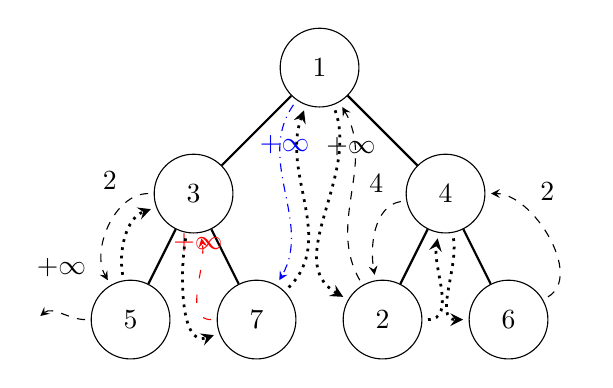
\begin{tikzpicture}[baseline=-2cm,scale=0.8]
        \node[circle,draw,minimum size=1cm] (1) at (0,0)  {$1$};
        \node[circle,draw,minimum size=1cm] (2) at (-2,-2){$3$};
        \node[circle,draw,minimum size=1cm] (3) at (2,-2) {$4$};
        \node[circle,draw,minimum size=1cm] (4) at (-3,-4){$5$};
        \node[circle,draw,minimum size=1cm] (5) at (1,-4) {$2$};
        \node[circle,draw,minimum size=1cm] (6) at (3,-4) {$6$};
        \node[circle,draw,minimum size=1cm] (7) at (-1,-4){$7$};
        % \node[label={7},circle,draw,minimum size=1cm] (7) at (3,-4) {$8$};
        % \node[label={9},circle,draw,minimum size=1cm] (9) at (-2,-6) {$1$};
        \tikzstyle{filho}=[thick]
        \tikzstyle{pred}=[->, shorten >= 2pt, shorten <= 2pt,
        dashed, >=stealth]
        \tikzstyle{sucessor}=[->, shorten >= 2pt, shorten <= 2pt,
        dotted, >=stealth, line width=0.35mm]
        % \tikzstyle{p4}=[->, shorten >= 2pt, shorten <= 2pt, dotted, >=stealth]
        \draw[filho] (1) -- (2);
        \draw[filho] (1) -- (3);
        \draw[filho] (2) -- (4);
        \draw[filho] (2) -- (7);
        \draw[filho] (3) -- (5);
        \draw[filho] (3) -- (6);
        \draw[pred] (6) edge[out=30,in=0]
        node[above=10pt] {$2$} (3);
        \draw[sucessor] (3) edge[out=280,in=180] (6);
        \draw[pred] (3) edge[out=190,in=100]
        node[above=10pt] {$4$} (5);
        \draw[sucessor] (5) edge[out=0,in=260] (3);
        \draw[pred] (5) edge[out=120,in=300]
        node[above=10pt] {$+\infty$} (1);
        \draw[sucessor] (1) edge[out=290,in=150] (5);
        \draw[pred, loosely dashed, red] (7) edge[out=180,in=280]
        node[red, above=10pt] {$+\infty$} (2);
        \draw[sucessor] (2) edge[out=260,in=200] (7);
        \draw[pred, blue, dashdotted] (1) edge[out=235,in=60]
        node[blue, above=10pt] {$+\infty$} (7);
        \draw[sucessor] (7) edge[out=45,in=250] (1);
        \draw[pred] (2) edge[out=180,in=120]
        node[above=10pt] {$2$} (4);
        \draw[sucessor] (4) edge[out=100,in=200] (2);
        \draw[pred] (4) edge[out=180,in=40]
        node[above=10pt] {$+\infty$} (-4.5, -4);
    \end{tikzpicture}
    \begin{tabular}{|c|c|c|c|c|}
        \hline
        &       &       & $\now = 1$                  \\
        $i$ & $x_0$ & $v$   & $\cert[i]$                  \\
        \hline
        $1$ & $6$   & $2$   & \textcolor{blue}{$+\infty$} \\

        $2$ & $3$   & $5$   & $+\infty$                   \\

        $3$ & $2$   & $1$   & $2$                         \\

        $4$ & $7$   & $4$   & $4$                         \\

        $5$ & $-2$  & $3$   & $+\infty$                   \\

        $6$ & $14$  & $0.5$ & $2$                         \\

        $7$ & $3$   & $1$   & \textcolor{red}{$+\infty$}  \\
        \hline
    \end{tabular}
    \caption[ABB após chamar \textsc{insert}]{Após chamar
        {\normalfont \textsc{insert}$(1, 4)$}, no instante $1$, o elemento $7$ foi
    inserido na árvore.
    O certificado do elemento $7$ foi criado e o
    certificado do seu sucessor, o elemento $1$, atualizado.}
    \label{fig:abb:insert}
\end{figure}

\begin{figure}[htb]
    \centering
    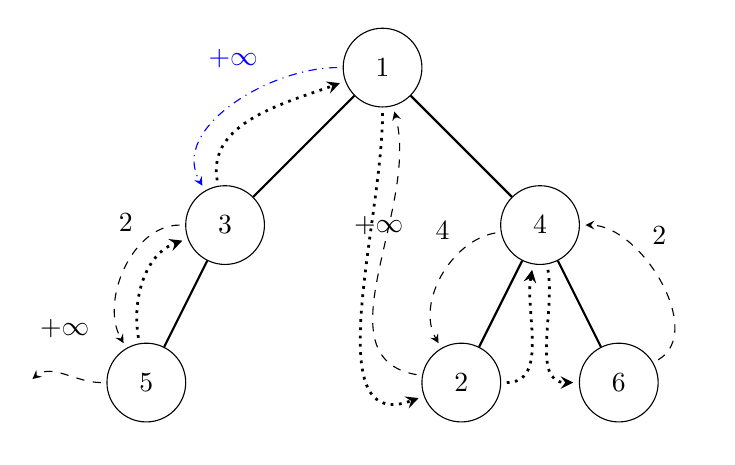
\begin{tikzpicture}[baseline=-2.25cm]
        \node[circle,draw,minimum size=1cm] (1) at (0,0)  {$1$};
        \node[circle,draw,minimum size=1cm] (2) at (-2,-2){$3$};
        \node[circle,draw,minimum size=1cm] (3) at (2,-2) {$4$};
        \node[circle,draw,minimum size=1cm] (4) at (-3,-4){$5$};
        \node[circle,draw,minimum size=1cm] (5) at (1,-4) {$2$};
        \node[circle,draw,minimum size=1cm] (6) at (3,-4) {$6$};
        % \node[label={7},circle,draw,minimum size=1cm] (7) at (3,-4) {$8$};
        % \node[label={8},circle,draw,minimum size=1cm] (8) at (-4,-6) {$4$};
        % \node[label={9},circle,draw,minimum size=1cm] (9) at (-2,-6) {$1$};
        \tikzstyle{filho}=[thick]
        \tikzstyle{pred}=[->, shorten >= 2pt, shorten <= 2pt,
        dashed, >=stealth]
        \tikzstyle{sucessor}=[->, shorten >= 2pt, shorten <= 2pt,
        dotted, >=stealth, line width=0.35mm]
        % \tikzstyle{p4}=[->, shorten >= 2pt, shorten <= 2pt, dotted, >=stealth]
        \draw[filho] (1) -- (2);
        \draw[filho] (1) -- (3);
        \draw[filho] (2) -- (4);
        \draw[filho] (3) -- (5);
        \draw[filho] (3) -- (6);
        \draw[pred] (6) edge[out=30,in=0]
        node[above=10pt] {$2$} (3);
        \draw[sucessor] (3) edge[out=280,in=180] (6);
        \draw[pred] (3) edge[out=190,in=120]
        node[above=10pt] {$4$} (5);
        \draw[sucessor] (5) edge[out=0,in=260] (3);
        \draw[pred] (5) edge[out=170,in=285]
        node[above=10pt] {$+\infty$} (1);
        \draw[sucessor] (1) edge[out=270,in=200] (5);
        \draw[pred, blue, dashdotted] (1) edge[out=180,in=120]
        node[blue, above=10pt] {$+\infty$} (2);
        \draw[sucessor] (2) edge[out=100,in=200] (1);
        \draw[pred] (2) edge[out=180,in=120]
        node[above=10pt] {$2$} (4);
        \draw[sucessor] (4) edge[out=100,in=200] (2);
        \draw[pred] (4) edge[out=180,in=40]
        node[above=10pt] {$+\infty$} (-4.5, -4);
    \end{tikzpicture}
    \begin{tabular}{|c|c|c|c|c|}
        \hline
        &       &       & $\now = 1.5$                \\
        $i$ & $x_0$ & $v$   & $\cert[i]$                  \\
        \hline
        $1$ & $6$   & $2$   & \textcolor{blue}{$+\infty$} \\

        $2$ & $3$   & $5$   & $+\infty$                   \\

        $3$ & $2$   & $1$   & $2$                         \\

        $4$ & $7$   & $4$   & $4$                         \\

        $5$ & $-2$  & $3$   & $+\infty$                   \\

        $6$ & $14$  & $0.5$ & $2$                         \\
        \hline
    \end{tabular}
    \caption[ABB após chamar \textsc{delete}]{Após chamar
        {\normalfont \textsc{delete}$(7)$} na árvore da Figura~\ref{fig:abb:insert}, o
    elemento $7$ foi retirado da árvore, a lista ligada foi
    ajustada, o certificado do seu sucessor, o elemento $1$, foi
    atualizado e o certificado do elemento $7$ foi destruído.}
    \label{fig:abb:delete}
\end{figure}

A operação \textsc{delete}$(i)$ consiste em recuperar o elemento
$i$, removê-lo da árvore binária balanceada de busca e da estrutura
que usamos para recuperá-lo, e depois removê-lo da fila com
prioridades. Após isso, basta atualizar o certificado de seu
sucessor, caso exista. Essa operação é ilustrada na Figura
\ref{fig:abb:delete} e implementada no Algoritmo \ref{abb:delete}.

\begin{figure}[htb]
    \centering
    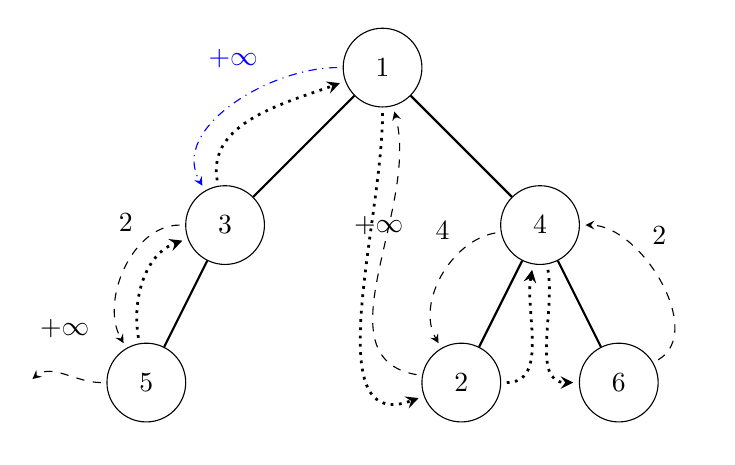
\begin{tikzpicture}[baseline=-2.25cm]
        \node[circle,draw,minimum size=1cm] (1) at (0,0)  {$1$};
        \node[circle,draw,minimum size=1cm] (2) at (-2,-2){$3$};
        \node[circle,draw,minimum size=1cm] (3) at (2,-2) {$4$};
        \node[circle,draw,minimum size=1cm] (4) at (-3,-4){$5$};
        \node[circle,draw,minimum size=1cm] (5) at (1,-4) {$2$};
        \node[circle,draw,minimum size=1cm] (6) at (3,-4) {$6$};
        % \node[label={7},circle,draw,minimum size=1cm] (7) at (3,-4) {$8$};
        % \node[label={8},circle,draw,minimum size=1cm] (8) at (-4,-6) {$4$};
        % \node[label={9},circle,draw,minimum size=1cm] (9) at (-2,-6) {$1$};
        \tikzstyle{filho}=[thick]
        \tikzstyle{pred}=[->, shorten >= 2pt, shorten <= 2pt,
        dashed, >=stealth]
        \tikzstyle{sucessor}=[->, shorten >= 2pt, shorten <= 2pt,
        dotted, >=stealth, line width=0.35mm]
        % \tikzstyle{p4}=[->, shorten >= 2pt, shorten <= 2pt, dotted, >=stealth]
        \draw[filho] (1) -- (2);
        \draw[filho] (1) -- (3);
        \draw[filho] (2) -- (4);
        \draw[filho] (3) -- (5);
        \draw[filho] (3) -- (6);
        \draw[pred] (6) edge[out=30,in=0]
        node[above=10pt] {$2$} (3);
        \draw[sucessor] (3) edge[out=280,in=180] (6);
        \draw[pred] (3) edge[out=190,in=120]
        node[above=10pt] {$4$} (5);
        \draw[sucessor] (5) edge[out=0,in=260] (3);
        \draw[pred] (5) edge[out=170,in=285]
        node[above=10pt] {$+\infty$} (1);
        \draw[sucessor] (1) edge[out=270,in=200] (5);
        \draw[pred, blue, dashdotted] (1) edge[out=180,in=120]
        node[blue, above=10pt] {$+\infty$} (2);
        \draw[sucessor] (2) edge[out=100,in=200] (1);
        \draw[pred] (2) edge[out=180,in=120]
        node[above=10pt] {$2$} (4);
        \draw[sucessor] (4) edge[out=100,in=200] (2);
        \draw[pred] (4) edge[out=180,in=40]
        node[above=10pt] {$+\infty$} (-4.5, -4);
    \end{tikzpicture}
    \begin{tabular}{|c|c|c|c|c|}
        \hline
        &       &       & $\now = 1.5$                \\
        $i$ & $x_0$ & $v$   & $\cert[i]$                  \\
        \hline
        $1$ & $6$   & $2$   & \textcolor{blue}{$+\infty$} \\

        $2$ & $3$   & $5$   & $+\infty$                   \\

        $3$ & $2$   & $1$   & $2$                         \\

        $4$ & $7$   & $4$   & $4$                         \\

        $5$ & $-2$  & $3$   & $+\infty$                   \\

        $6$ & $14$  & $0.5$ & $2$                         \\
        \hline
    \end{tabular}
    \caption[ABB após chamar \textsc{delete}]{Após chamar
        {\normalfont \textsc{delete}$(7)$} na árvore da Figura~\ref{fig:abb:insert}, o
    elemento $7$ foi retirado da árvore, a lista ligada foi
    ajustada, o certificado do seu sucessor, o elemento $1$, foi
    atualizado e o certificado do elemento $7$ foi destruído.}
    \label{fig:abb:delete}
\end{figure}
